\chapter{results}\label{results}

\section{ghsep}\label{ghsep}
The trained random forests reaches an area under the ROC-curve (???) 
of XXXX, as can be seen in figure \ref{fig:gh_roc}.

\begin{figure}
    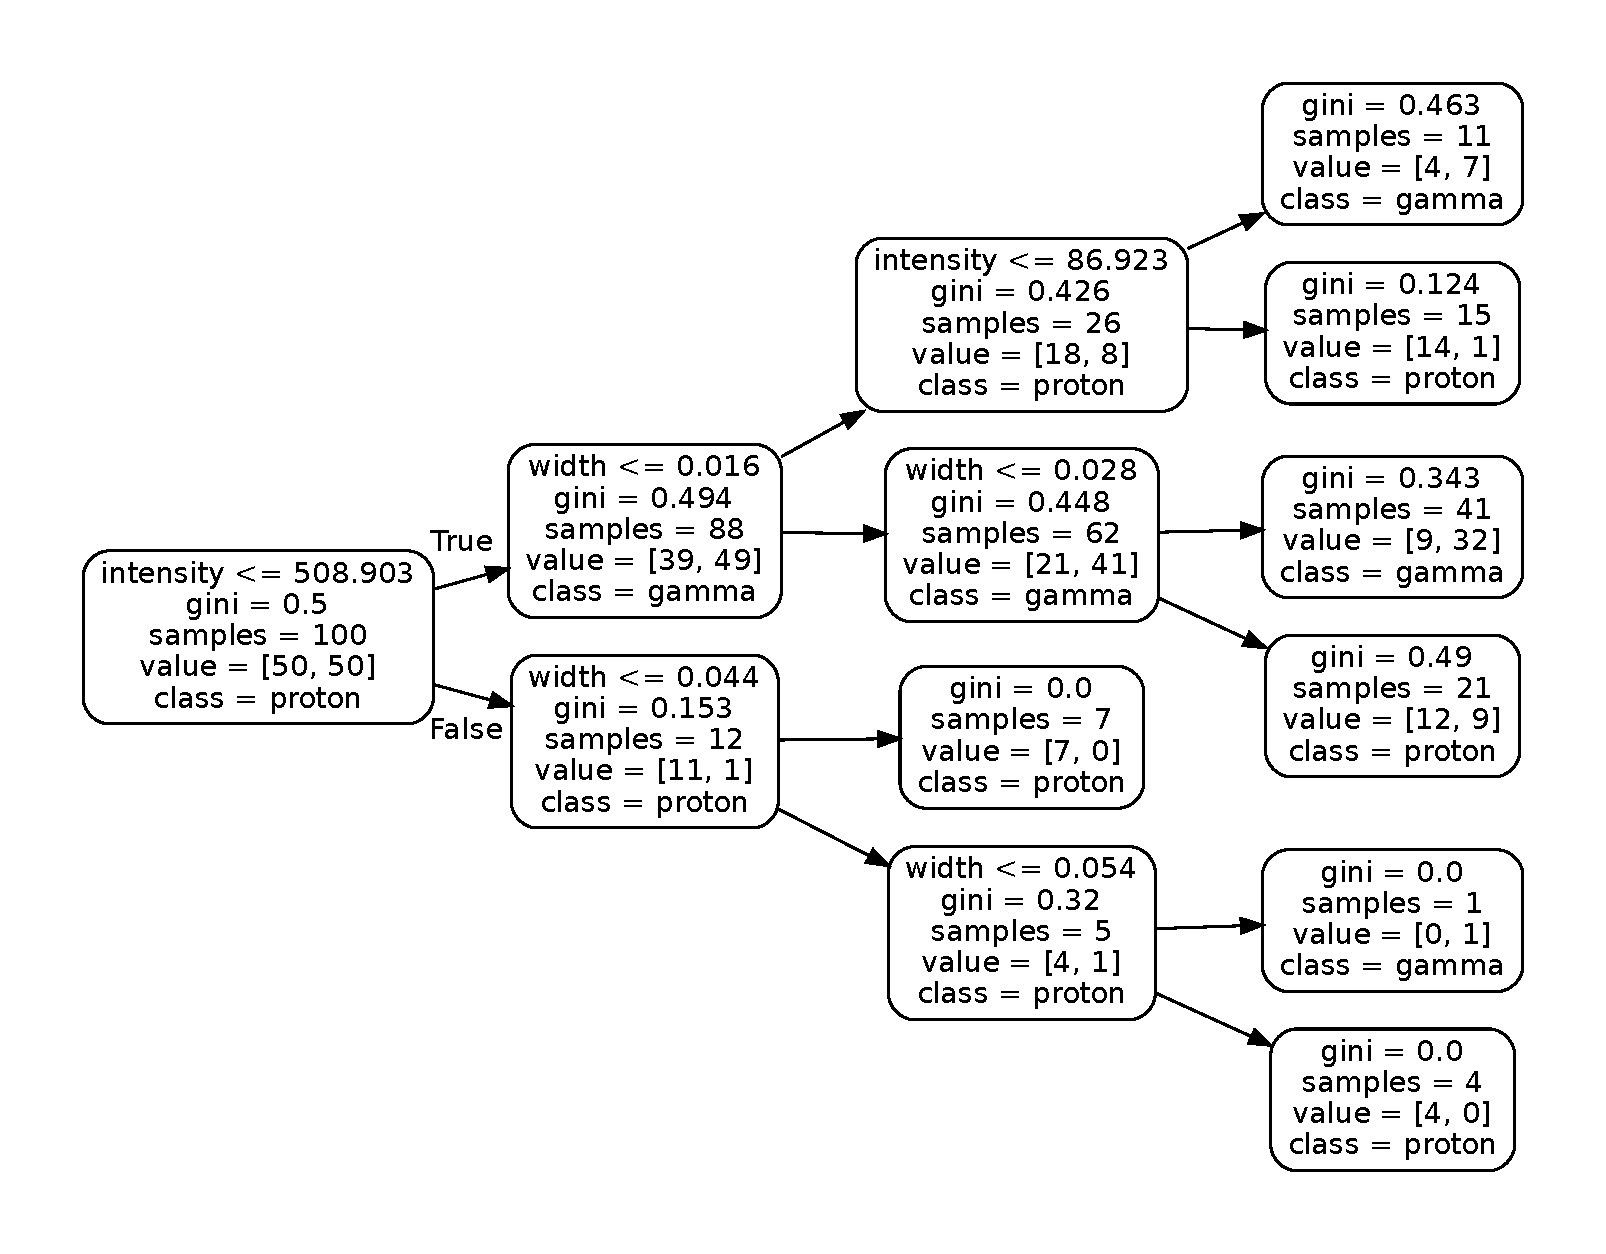
\includegraphics[width=.8\textwidth]{Plots/decision_tree.pdf}
    \caption{ROC for the gamma/hardon seperation on the cross validated training set 
    consisting of XXX proton events and YYY diffuse gamma events.}
    \label{fig:gh_roc}
\end{figure}

The feature importance, as defined in chapter XXX, is shown in \ref{fig:gh_features}.
\begin{figure}
    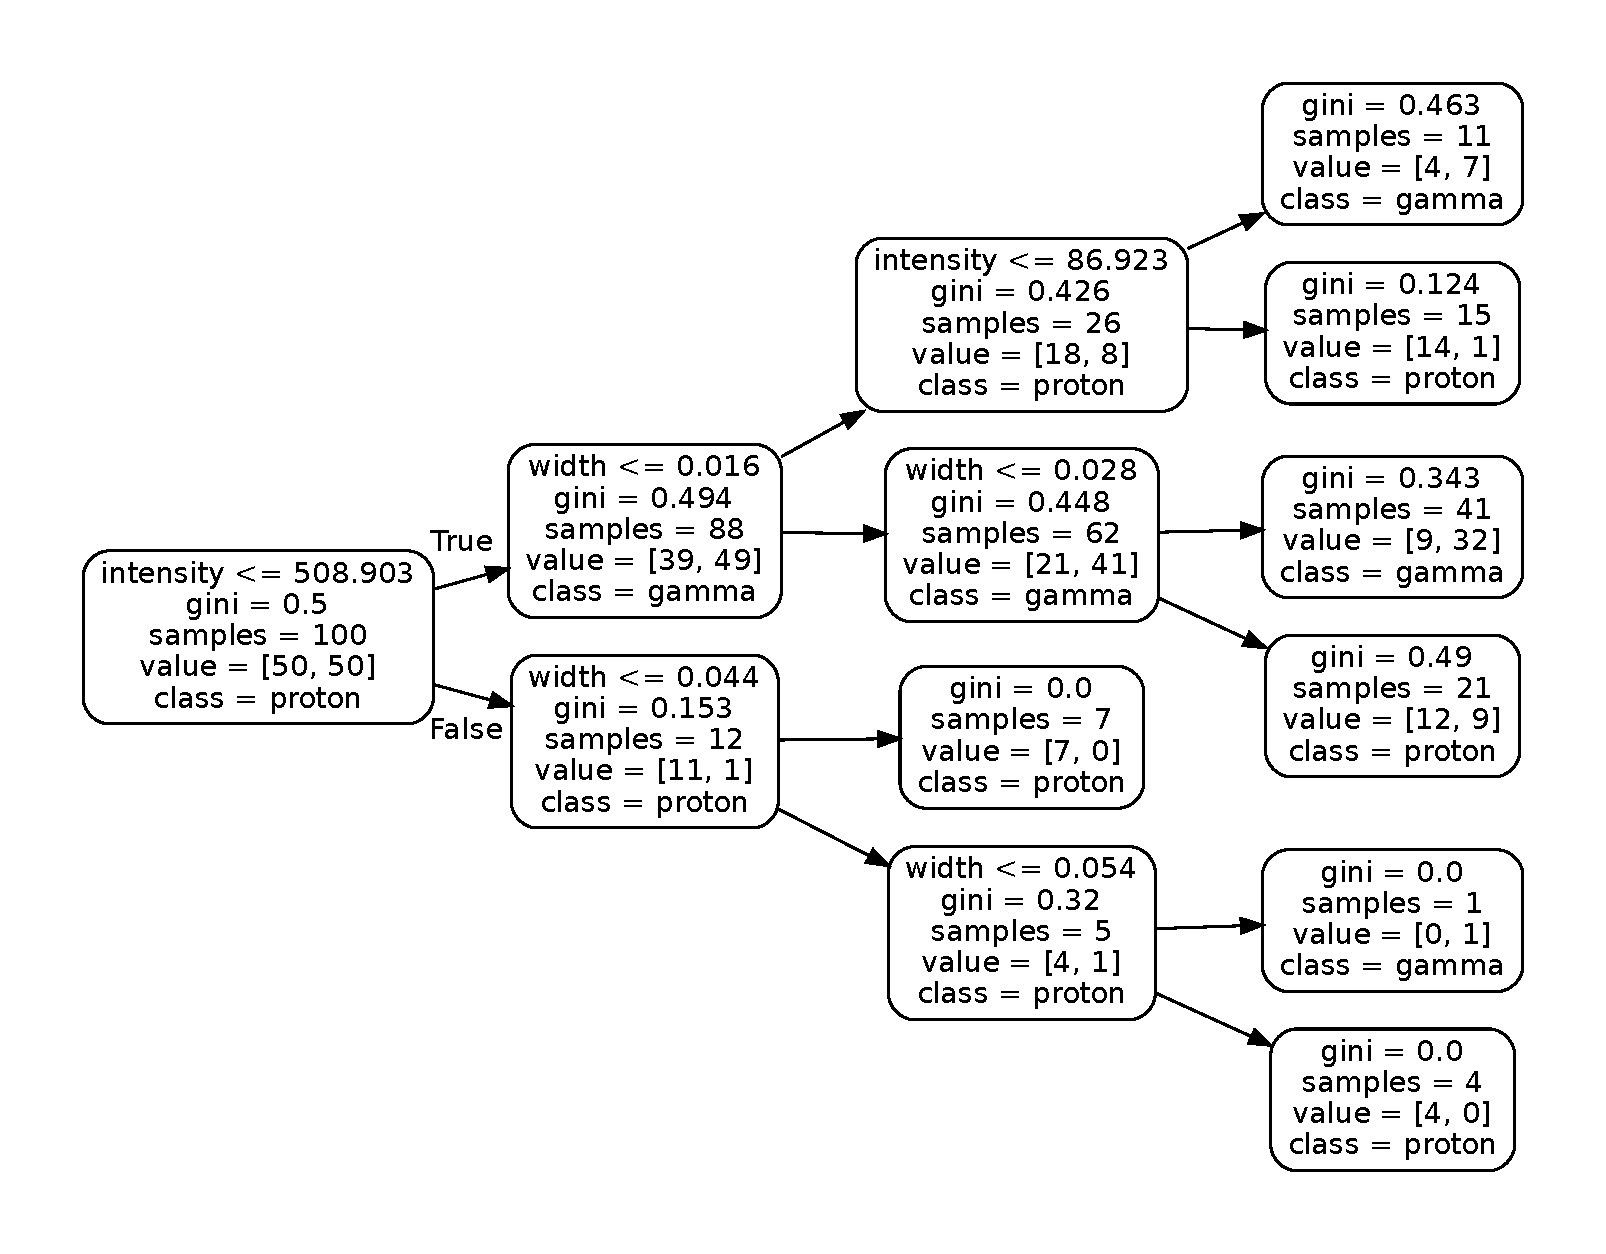
\includegraphics[width=.8\textwidth]{Plots/decision_tree.pdf}
    \caption{Feature importance for the gamma/hardon separation.}
    \label{fig:gh_features}
\end{figure}


Applied to our clean testset of pointlike gammas, we get:
.....
sowas wie der zweite plot da machen.

